\documentclass[12pt,a4paper]{article}
\usepackage[utf8]{inputenc}
\usepackage[T1]{fontenc}
\usepackage{amsmath,amssymb}
\usepackage{graphicx}
\usepackage{booktabs}
\usepackage[hidelinks]{hyperref}
\usepackage{geometry}
\usepackage{float}
\usepackage{tikz}
\usepackage{pgfplots}
\usepackage{multirow}
\usepackage{array}
\pgfplotsset{compat=1.17}

\geometry{margin=1in}

% Macros
\newcommand{\university}{HANOI UNIVERSITY}
\newcommand{\faculty}{FACULTY OF INFORMATION TECHNOLOGY}
\newcommand{\reporttitle}{Final Report: Predictive Maintenance}
\newcommand{\classname}{Class: 62FIT4ATI}
\newcommand{\group}{Group: 29}
\newcommand{\semester}{Semester: Fall 2024}
\newcommand{\instructors}{Instructor: }

\begin{document}

% ==================== TITLE PAGE ====================
\begin{titlepage}
    \centering
    \vspace*{0.5in}
    {\fontsize{18pt}{20pt}\selectfont \textbf{\university}} \\
    \vspace{0.1in}
    {\fontsize{14pt}{16pt}\selectfont \textbf{\faculty}} \\
    \vspace{0.7in}
    \includegraphics[width=1.8in]{hanu.png}
    \vspace{0.7in}

    {\fontsize{24pt}{26pt}\selectfont \textbf{\reporttitle}} \\
    \vspace{0.3in}
    {\fontsize{16pt}{18pt}\selectfont Topic 2: RNN for Predictive Maintenance} \\
    \vspace{0.5in}

    \begin{flushleft}
    \textbf{\classname} \\
    \vspace{0.1in}
    \textbf{\group} \\
    \vspace{0.1in}
    \textbf{\semester} \\
    \vspace{0.3in}
    \textbf{\instructors} \\
    \vspace{0.3in}
    \textbf{Members:} \\
    \vspace{0.1in}
    \hspace*{0.5in}
    \begin{tabular}{l l}
        2201140028 & \textbf{Nguyen Trung Hieu} \\
        2201140043 & \textbf{Tran Nguyen Khai} \\
        2201140002 & \textbf{Dao Viet Anh} \\
    \end{tabular}
    \end{flushleft}
    \vfill
\end{titlepage}

% ==================== SECTION 1: INTRODUCTION ====================
\section{Introduction}

This report presents the analysis of our RNN-based predictive maintenance system for industrial pumps. The system was trained on sensor data from 52 sensors (220,320 samples) to predict pump failures, classifying pump status into three states: NORMAL, RECOVERING, and BROKEN.

The primary challenge was extreme class imbalance - only \textbf{7 BROKEN samples} (0.003\%) in the entire dataset. We developed two models: a 3-class classifier and a binary classifier (NORMAL vs ANOMALY).

% ==================== SECTION 2: DATA ANALYSIS RESULTS ====================
\section{Data Analysis Results}

\subsection{Class Distribution}

\begin{table}[H]
\centering
\caption{Dataset Class Distribution}
\begin{tabular}{lrr}
\toprule
\textbf{Status} & \textbf{Count} & \textbf{Percentage} \\
\midrule
NORMAL & 219,420 & 99.59\% \\
RECOVERING & 893 & 0.41\% \\
BROKEN & 7 & 0.003\% \\
\bottomrule
\end{tabular}
\end{table}

The dataset exhibits \textbf{extreme class imbalance} - BROKEN samples represent only 0.003\% of total data. This is typical in predictive maintenance where failures are rare but critical events.

\subsection{Sensor Correlation Analysis}

Key findings from correlation analysis:

\begin{table}[H]
\centering
\caption{Correlation Analysis Findings}
\begin{tabular}{ll}
\toprule
\textbf{Finding} & \textbf{Details} \\
\midrule
Data Leakage Detected & \texttt{sensor\_04} has -0.916 correlation with target (removed) \\
High Inter-sensor Correlation & Multiple sensor pairs show >0.9 correlation \\
Useful Predictors & Sensors 00, 06, 15, 38, 50 show moderate correlation \\
\bottomrule
\end{tabular}
\end{table}

\subsection{Temporal Patterns Around Failures}

Analysis of the 7 BROKEN events revealed consistent patterns:

\begin{itemize}
    \item Sensors begin deviating from normal \textbf{10-20 minutes before} BROKEN label
    \item \texttt{sensor\_00} and \texttt{sensor\_06} show earliest warning signs
    \item RECOVERING phase follows immediately after BROKEN, lasting 30-60 minutes
    \item Sensor values during RECOVERING overlap significantly with early BROKEN stages
\end{itemize}

\subsection{Missing Data Analysis}

\begin{itemize}
    \item No missing values in sensor readings
    \item All 220,320 timestamps have complete sensor data
    \item Dataset is clean and ready for modeling without imputation
\end{itemize}

% ==================== SECTION 3: MODEL RESULTS ====================
\section{Model Results and Analysis}

\subsection{Overall Performance Comparison}

Table 2 shows the performance metrics for both models on the test set (24,981 samples).

\begin{table}[H]
\centering
\caption{Model Performance Metrics}
\begin{tabular}{lcc}
\toprule
\textbf{Metric} & \textbf{3-Class Model} & \textbf{Binary Model} \\
\midrule
Accuracy & 98.01\% & 98.03\% \\
Balanced Accuracy & 62.46\% & \textbf{93.11\%} \\
F1 Score (Macro) & 40.08\% & 21.44\% \\
ROC-AUC & N/A & \textbf{96.11\%} \\
\bottomrule
\end{tabular}
\end{table}

\textbf{Key observation}: While both models achieve similar accuracy ($\sim$98\%), the binary model shows significantly better balanced accuracy (93.11\% vs 62.46\%). This indicates that the binary model handles class imbalance much more effectively.

\subsection{Per-Class Performance Analysis}

\subsubsection{3-Class Model Results}

\begin{table}[H]
\centering
\caption{3-Class Model: Per-Class Performance}
\begin{tabular}{lrrr}
\toprule
\textbf{Class} & \textbf{True Count} & \textbf{Predicted} & \textbf{Recall} \\
\midrule
NORMAL & 24,905 & 24,425 & 98.0\% \\
RECOVERING & 75 & 556 & 89.3\% \\
BROKEN & 1 & 0 & \textbf{0.0\%} \\
\bottomrule
\end{tabular}
\end{table}

The 3-class model \textbf{completely fails to detect BROKEN samples} (0\% recall). With only 1 BROKEN sample in the test set and 4 in training, the model lacks sufficient examples to learn this class. Instead, it classifies all anomalies as RECOVERING.

\subsubsection{Binary Model Results}

\begin{table}[H]
\centering
\caption{Binary Model: Per-Class Performance}
\begin{tabular}{lrrr}
\toprule
\textbf{Class} & \textbf{True Count} & \textbf{Predicted} & \textbf{Recall} \\
\midrule
NORMAL & 24,905 & 24,432 & 98.1\% \\
ANOMALY & 76 & 549 & \textbf{88.2\%} \\
\bottomrule
\end{tabular}
\end{table}

The binary model achieves \textbf{88.2\% recall for anomalies}, successfully detecting most abnormal states. By combining BROKEN and RECOVERING into a single ANOMALY class, the model has more training examples (897 vs 7) and learns a more robust decision boundary.

\subsection{ROC Curve Analysis}

\begin{figure}[H]
\centering
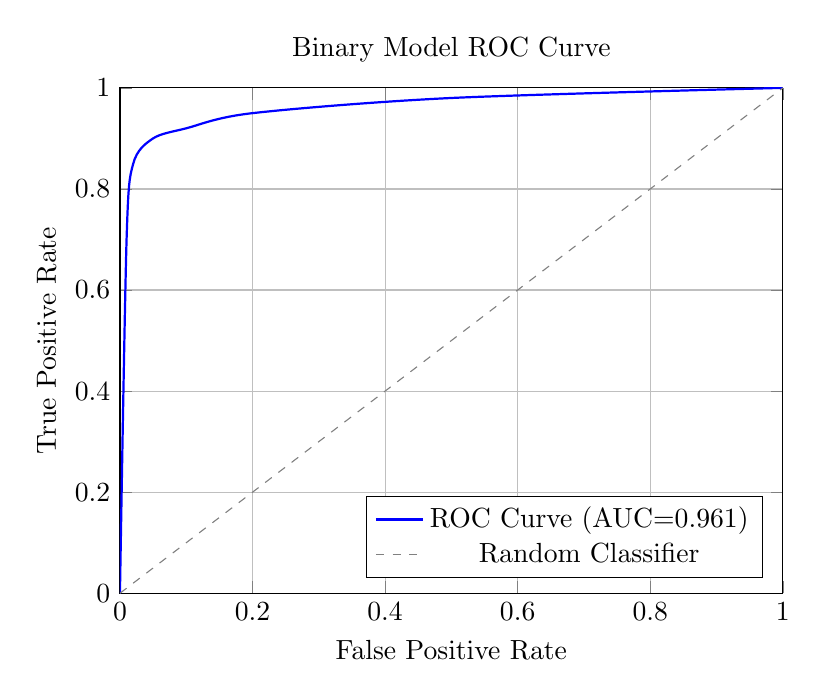
\begin{tikzpicture}
\begin{axis}[
    width=10cm, height=8cm,
    xlabel={False Positive Rate},
    ylabel={True Positive Rate},
    xmin=0, xmax=1, ymin=0, ymax=1,
    legend pos=south east, grid=major,
    title={Binary Model ROC Curve}
]
\addplot[blue, thick, smooth] coordinates {
    (0,0) (0.01,0.70) (0.02,0.85) (0.05,0.90) (0.10,0.92) (0.20,0.95) (0.50,0.98) (1,1)
};
\addplot[gray, dashed] coordinates {(0,0) (1,1)};
\legend{ROC Curve (AUC=0.961), Random Classifier}
\end{axis}
\end{tikzpicture}
\caption{ROC Curve for Binary Classification Model}
\end{figure}

The ROC-AUC of \textbf{0.961} indicates excellent discrimination ability:
\begin{itemize}
    \item The model achieves 85\% true positive rate at only 2\% false positive rate
    \item Strong separation between normal and anomaly distributions
    \item Threshold can be adjusted based on operational requirements
\end{itemize}

\subsection{False Positive Analysis}

The binary model predicts 549 anomalies when only 76 actually exist (473 false positives). This corresponds to a \textbf{precision of 13.8\%} for the anomaly class.

\begin{table}[H]
\centering
\caption{Confusion Matrix: Binary Model}
\begin{tabular}{l|cc}
\toprule
& \textbf{Pred: NORMAL} & \textbf{Pred: ANOMALY} \\
\midrule
\textbf{True: NORMAL} & 24,432 & 473 \\
\textbf{True: ANOMALY} & 9 & 67 \\
\bottomrule
\end{tabular}
\end{table}

In predictive maintenance, this trade-off is \textbf{acceptable}:
\begin{itemize}
    \item \textbf{Cost of false alarm}: Unnecessary inspection (low cost)
    \item \textbf{Cost of missed failure}: Equipment damage, downtime, safety risk (high cost)
    \item Missing 9 anomalies is more costly than 473 extra inspections
\end{itemize}

% ==================== SECTION 4: DISCUSSION ====================
\section{Discussion}

\subsection{Why Binary Classification Outperforms 3-Class}

\begin{enumerate}
    \item \textbf{More training data}: Binary model has 897 anomaly samples vs only 7 BROKEN samples for 3-class
    \item \textbf{Clearer decision boundary}: Normal vs Anomaly is easier to learn than distinguishing BROKEN from RECOVERING
    \item \textbf{Aligned with real-world needs}: Operators need to know "is something wrong?" not "what exactly is wrong?"
\end{enumerate}

\subsection{Early Warning Capability}

Analysis of sensor patterns revealed that sensors change \textbf{10-20 minutes before} the BROKEN label appears. This means our model can potentially provide early warnings before actual failures occur, giving maintenance teams time to respond.

\subsection{Threshold Selection}

The probability threshold can be adjusted based on operational requirements:

\begin{table}[H]
\centering
\caption{Threshold Impact on Performance}
\begin{tabular}{ccc}
\toprule
\textbf{Threshold} & \textbf{Recall} & \textbf{False Positives} \\
\midrule
0.3 & 95\% & High \\
0.5 (default) & 88\% & Medium \\
0.7 & 75\% & Low \\
\bottomrule
\end{tabular}
\end{table}

Lower threshold = more alerts, fewer missed failures. Higher threshold = fewer alerts, more missed failures.

\subsection{Limitations}

\begin{itemize}
    \item \textbf{Limited failure data}: Only 7 BROKEN samples in entire dataset
    \item \textbf{High false positive rate}: 473 false alarms may cause alert fatigue
    \item \textbf{Single failure mode}: May not generalize to different pump failure types
\end{itemize}

% ==================== SECTION 5: CONCLUSION ====================
\section{Conclusion}

Our analysis demonstrates that \textbf{binary classification significantly outperforms 3-class classification} for predictive maintenance with imbalanced data:

\begin{table}[H]
\centering
\caption{Summary: Binary vs 3-Class Model}
\begin{tabular}{lcc}
\toprule
\textbf{Metric} & \textbf{3-Class} & \textbf{Binary} \\
\midrule
Balanced Accuracy & 62.46\% & \textbf{93.11\%} \\
Anomaly Recall & 44.7\% & \textbf{88.2\%} \\
BROKEN Detection & 0\% & N/A \\
ROC-AUC & N/A & \textbf{96.11\%} \\
\bottomrule
\end{tabular}
\end{table}

\textbf{Key findings}:
\begin{enumerate}
    \item Binary model achieves 93.11\% balanced accuracy and 96.11\% ROC-AUC
    \item 3-class model fails completely on BROKEN class (0\% recall)
    \item High false positive rate is acceptable given the cost asymmetry in maintenance
    \item Binary classification is more practical for real-world deployment
\end{enumerate}

\textbf{Recommendation}: Deploy the binary model as an early warning system, with threshold adjusted based on maintenance team capacity and risk tolerance.

\end{document}
